\subsection{Controlador de pantalla VGA}
\label{vga}

\begin{figure}[H]
	\centering
	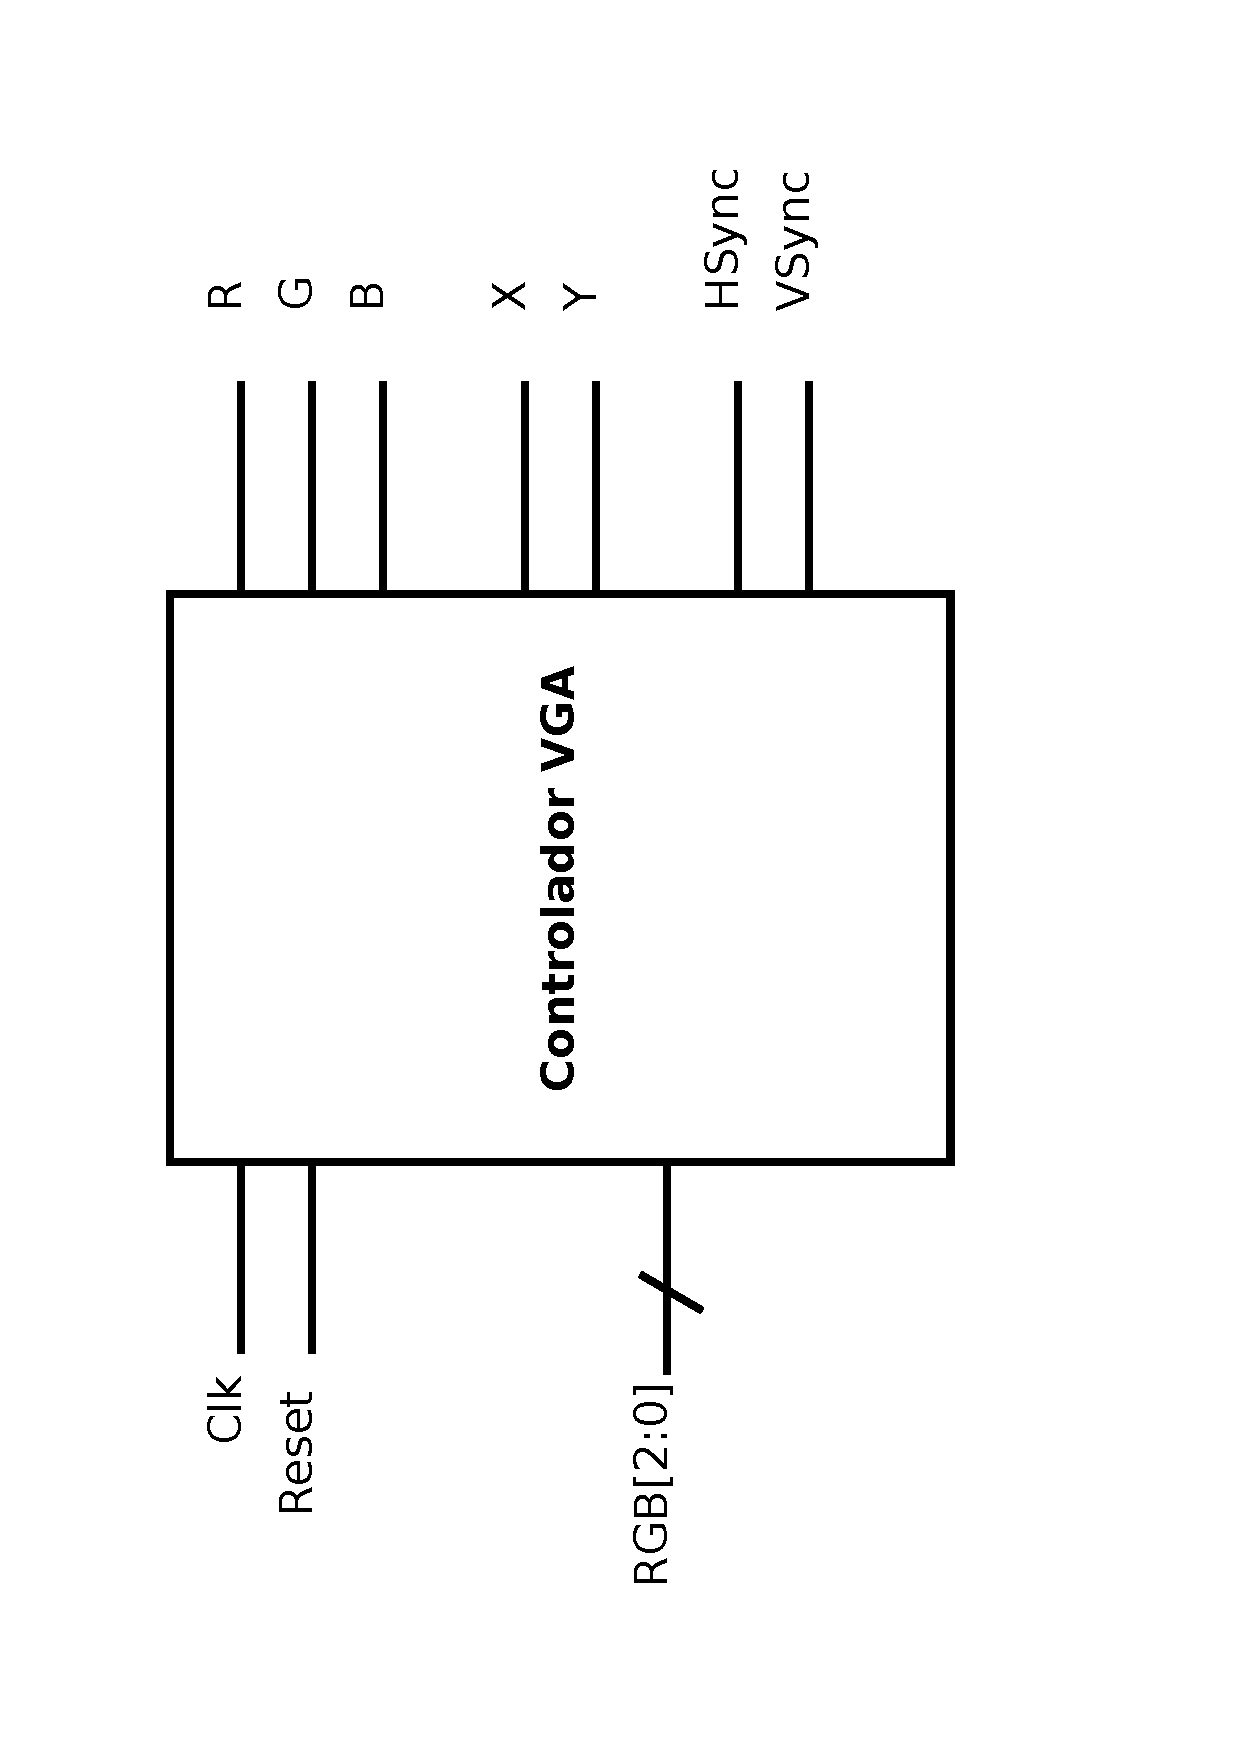
\includegraphics[width=0.4\textwidth, angle=-90] {vga_block.pdf}
	\caption{Interfaz del controlador de pantalla VGA}\label{fig:vgaBlock}
\end{figure}

El controlador de pantalla VGA se encarga de generar el patrón de ondas necesario para mostrar los gráficos del juego en una pantalla externa.

\subsubsection{Descripción Funcional}

El estándar VGA usa tres señales analógicas para codificar el color de cada píxel (R, G y B en la figura \ref{fig:vgaBlock}) y dos señales de sincronización que indican el fin de línea $HSync$ y fin de pantalla $VSync$). Para la implementación del controlador se ha usado una frecuencia de 25 MHz, que genera una resolución de 640 x 480 píxeles a una tasa de refresco de 60 Hz.

Para formar la imagen deseada en la pantalla, el controlador VGA accede a la información de color de cada píxel de manera similar a una memoria: las señales x e y indican la posición del píxel al bloque \hyperref[formatoVGA]{Formato VGA}, que devuelve el valor del color a través del bus $RGB$. 

Dado que la placa de desarrollo \emph{Spartan 3E Starter Kit} contiene un conversor digital a analógico (DAC) de un sólo bit para las señales $R$,$G$ y $B$, sólo es posible mostrar 8 colores diferentes en la pantalla.

\subsubsection{Implementación}

Las señales VGA \textit{HSync} y \textit{VSync} son siempre periódicas y están controladas por dos contadores en cascada: \textit{HCount} (con valores de 0 a 800) y \textit{Vcount} (0 a 521). El contador horizontal \textit{HCount} proporciona un marco temporal para mostrar los 640 píxeles que hay en cada línea de la pantalla, terminando cada ciclo con pulso bajo en \textit{HSync}, indicando que el monitor debe comenzar una nueva linea. 

Cada vez que se termina una línea, el contador vertical \textit{VCount} aumenta su valor hasta completar una pantalla (480 líneas). Entonces, un pulso bajo en \textit{VSync} indica al monitor que debe comenzar una nueva imagen.

Estos contadores usan un \emph{prescaler} de 1 bit, ya que la señal \textit{clk} tiene una frecuencia de 50 MHz pero la interfaz con la pantalla está configurada a 25 MHz.


